\documentclass[tikz,border=10pt]{standalone}
\usepackage{amsmath}
\begin{document}
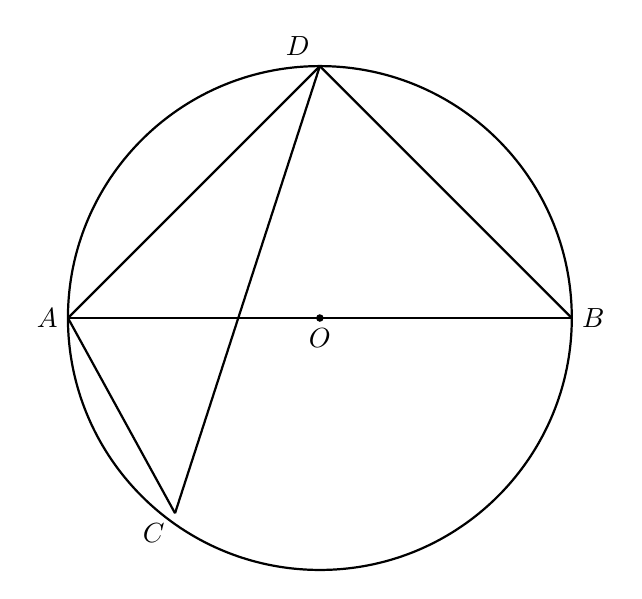
\begin{tikzpicture}[scale=0.04, line width=0.8pt]
  % Circle centre O and radius
  \coordinate (O) at (0,0);
  \coordinate (A) at (-80,0);
  \coordinate (B) at (80,0);
  \coordinate (D) at (0,80);
  \coordinate (C) at (-46,-62);

  % Circle
  \draw (O) circle (80);

  % Edges
  \draw (A) -- (B);
  \draw (A) -- (D);
  \draw (D) -- (B);
  \draw (A) -- (C);
  \draw (D) -- (C);

  % Centre point
  \fill (O) circle (1.2);

  % Labels
  \node[above left] at (D) {$D$};
  \node[left] at (A) {$A$};
  \node[right] at (B) {$B$};
  \node[below] at (O) {$O$};
  \node[below left] at (C) {$C$};
\end{tikzpicture}
\end{document}
